\subsection{Análisis de Señales Moduladas BPSK}
La reestructuración del diagrama de bloques para soportar la modulación BPSK se consolidó de forma exitosa. Las simulaciones en el dominio del tiempo y de la frecuencia revelan contrastes críticos entre el procesamiento de una señal modulada completa (RF) y su equivalente en banda base (EC).

\begin{figure}[H]
    \centering
    \subfloat[Señales en el dominio del tiempo.]{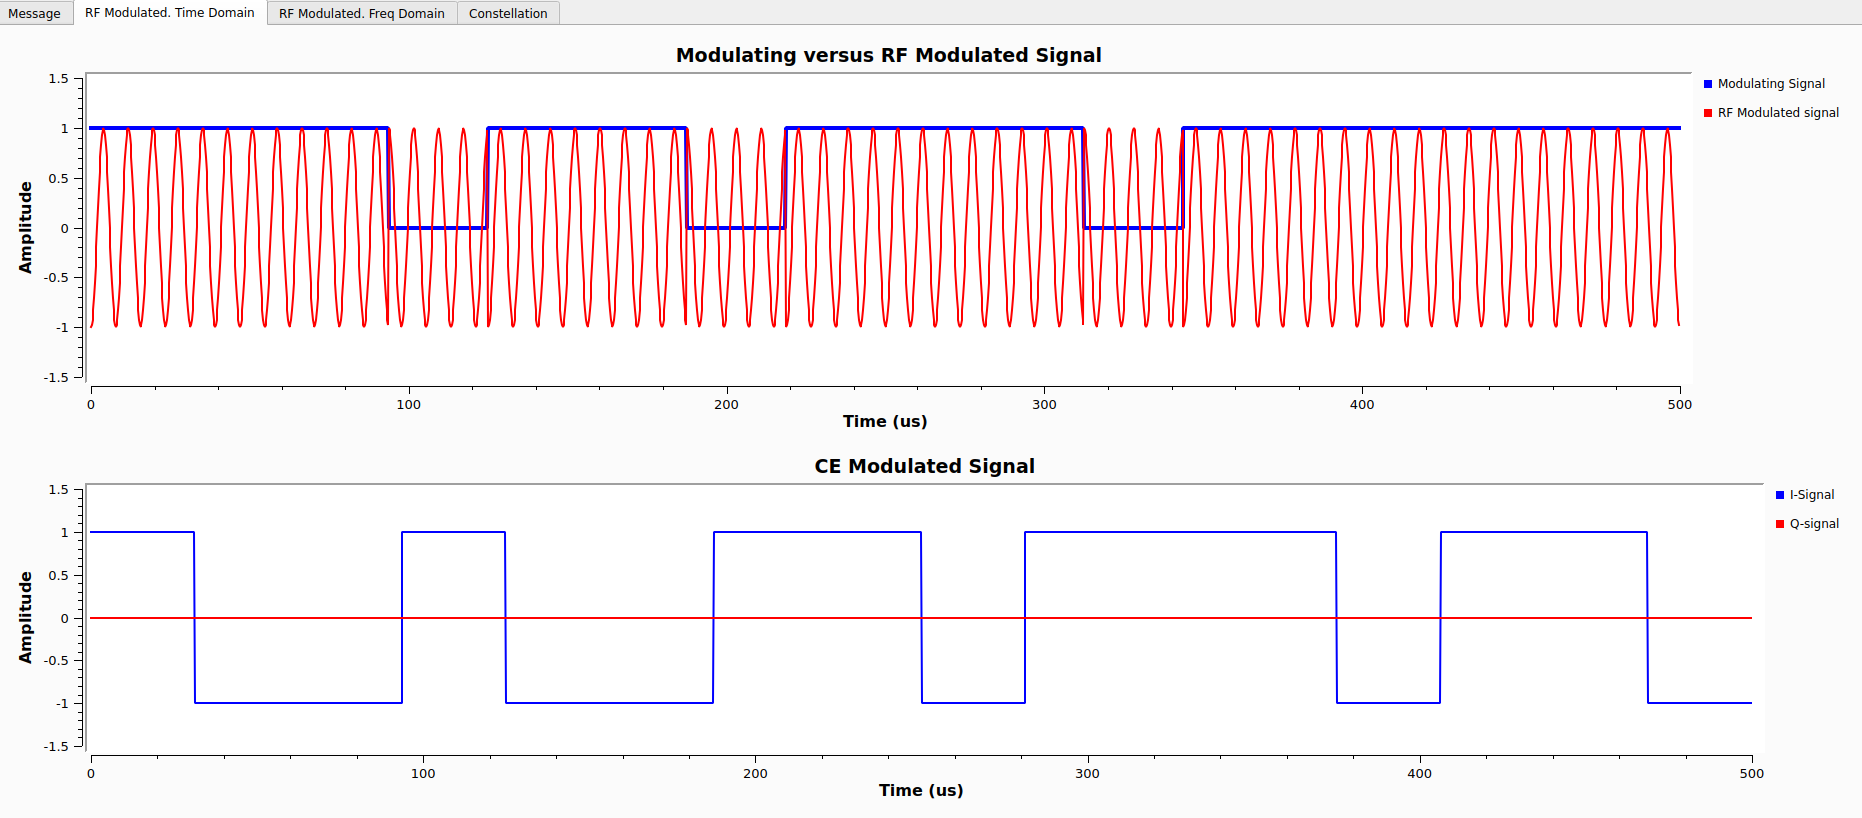
\includegraphics[width=0.48\linewidth]{imagenes/bpsk_tiempo.png}\label{fig:bpsk_a}}
    \hfill
    \subfloat[Espectro desplazado a una portadora de $500 \text{ kHz}$.]{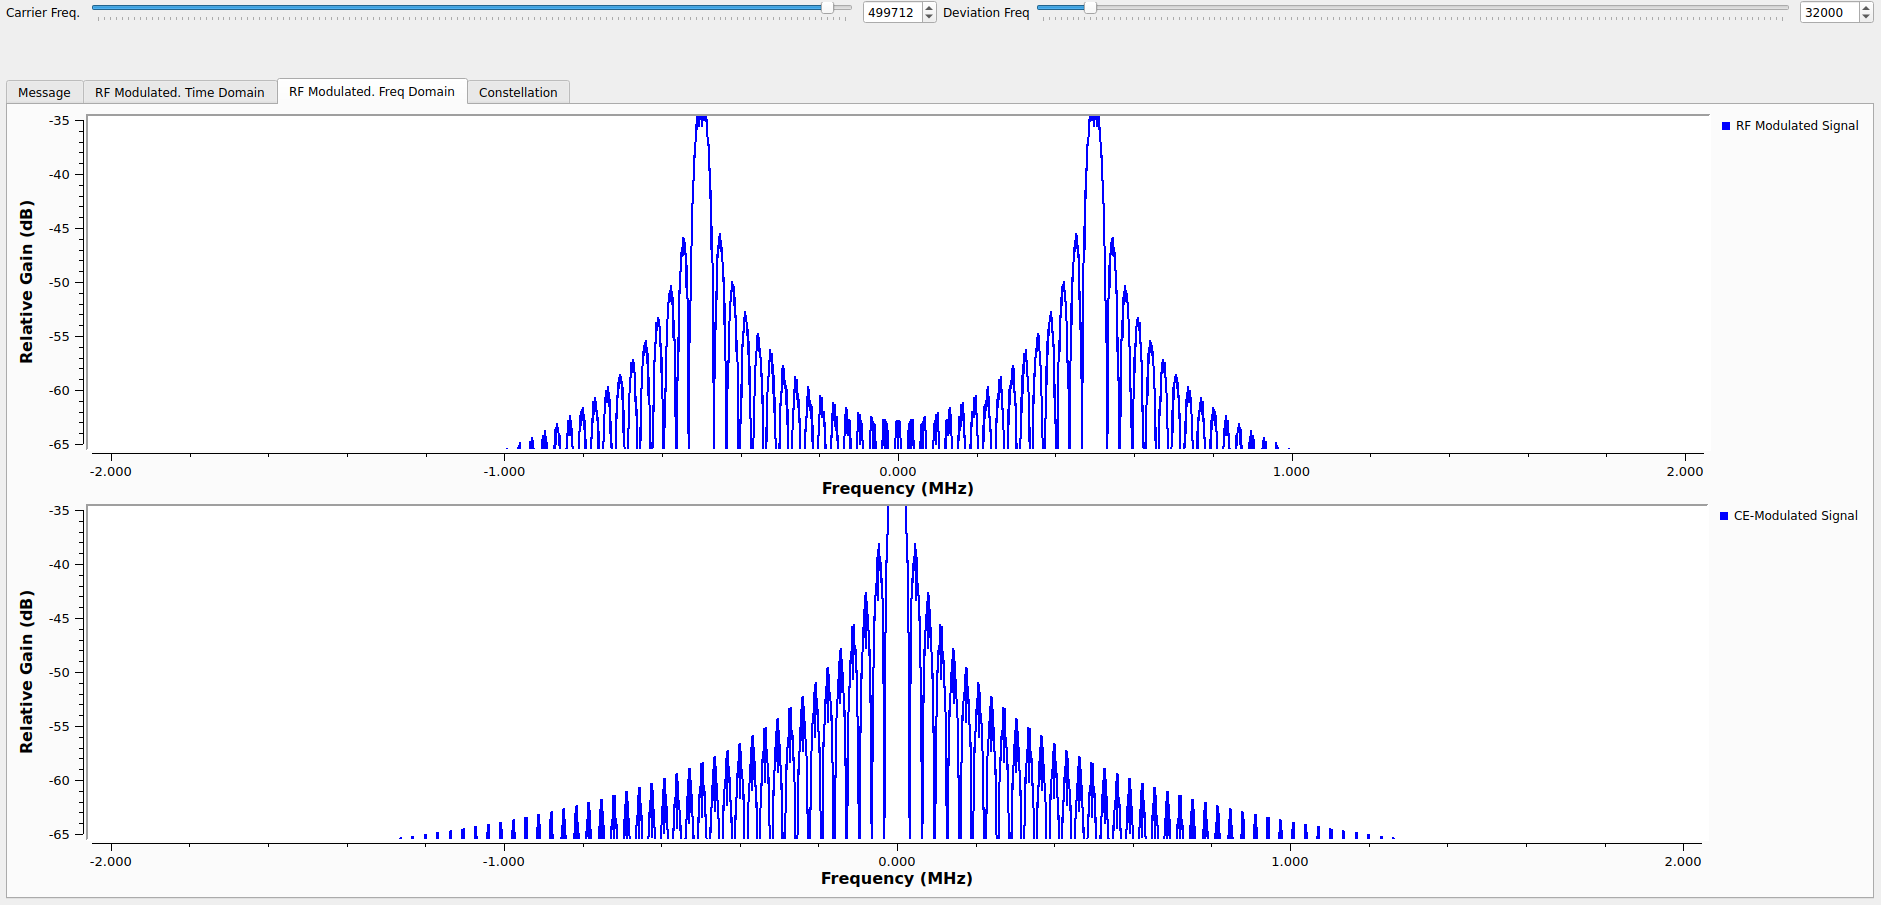
\includegraphics[width=0.48\linewidth]{imagenes/bpsk_frecuencia_var.png}\label{fig:bpsk_b}}
    \caption{Simulación BPSK comparando la versión RF (superior) y la EC (inferior).}
    \label{fig:simulacion_bpsk}
\end{figure}

A partir de la Figura \ref{fig:bpsk_a}, el bloque \textit{QT GUI Time Sink} evidencia cómo la señal RF efectúa transiciones abruptas en los cruces por cero para cumplir con el desfase de $\pi$. Sin embargo, la Figura \ref{fig:bpsk_b} aporta el resultado analítico más sustancial: al someter el sistema a una variación de portadora, el espectro de la señal RF se traslada forzosamente a dichas frecuencias (en este caso, cerca de los $500 \text{ kHz}$). 

Este desplazamiento obliga a utilizar un parámetro \textit{Samples Per Symbol (SPS)} desproporcionadamente alto para cumplir con el criterio de Nyquist sobre la frecuencia portadora y evitar el solapamiento (\textit{aliasing}). En drástico contraste, el espectro de la Envolvente Compleja permanece invariante y centrado en $0 \text{ Hz}$, demostrando que procesar la información analítica extraída de los cambios de estado (componentes I y Q) reduce exponencialmente la carga computacional en simulaciones.